\section{Auswertung}
\label{sec:Auswertung}
Die Graphen wurden sowohl mit Matplotlib \cite{matplotlib} als auch NumPy \cite{numpy} erstellt. Die
Fehlerrechnung wurde mithilfe von Uncertainties \cite{uncertainties} durchgeführt.


\subsection{Die Bestimmung der Detektorkenngrößen mithilfe des Spektrums von $^{152}$Eu} 
\begin{figure}
	\centering
	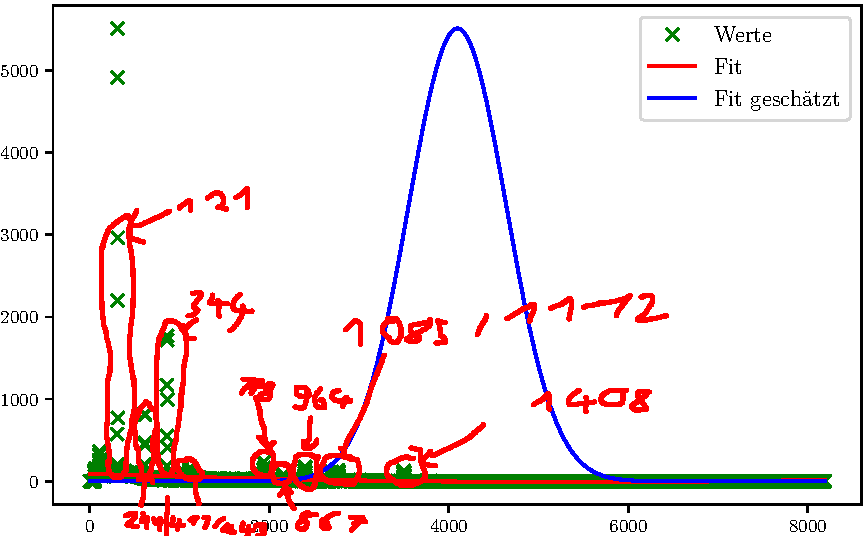
\includegraphics[width=\linewidth-70pt,height=\textheight-70pt,keepaspectratio]{build/EU152.pdf}
	\caption{Das Spektrum eines $^{152}$Eu-Strahlers, bei einer Messzeit von $\SI{4740}{\second}$, mit der Kanalnummer $K$ und der Anzahl der im Kanal nachgewiesenen Ereignisse $N$.}
	\label{fig:1}
\end{figure}
\begin{table}
	\centering
	\caption{Die Parameter der gefitteten Peaks des Spektrums von $^{152}$Eu mit den zugeordneten Energien.}
	\input{build/a.tex}
\end{table}


\subsubsection{Bestimmung der Energiekalibrierung des Spektrometers}
\label{subsec:EnergieKali}
\begin{figure}
	\centering
	\includegraphics[width=\linewidth-70pt,height=\textheight-70pt,keepaspectratio]{build/EnergieKali.pdf}
	\caption{Die Energie $E_\gamma$ gegen die Kanalnummer $K$ aufgetragen, wobei die Unsicherheit des einzelnen Wertepaares sich durch die Unsicherheit der Position der Gaußkurve und der Unsicherheit des Literaturwertes für $E_\gamma$ ergibt.}
	\label{fig:E}
\end{figure}
Zunächst wird den einzelnen Kanälen mithilfe einer Energiekalibrierung eine zugehörige Energie zugeordnet. Um eine möglichst exakte Kalibrierung vornehmen zu können wird $^{152}$Eu als Kalibrationsstrahler verwendet, da dieser ein reichhaltiges Spektrum besitzt. Zur Kalibrierung werden zunächst die einzelnen Vollenergiepeaks des Spektrums herausgesucht und jeweils mit einem Fit der Form
\begin{equation}
    N(K)=a \cdot \exp\left(\frac{1}{2}\left( \frac{K-b}{\sigma}\right)^2\right) +c
\end{equation}
ohne Gewichtung gefittet. Es ergeben sich die Werte in Tabelle \ref{tab:a}. Es werden alle Wertepaare, die zu einem Peak gehören, welcher durch Emissionen mit einer Wahrscheinlichkeit von unter $\SI{2}{\percent}$ zustande kommt, für die weiteren Fits ignoriert. Die Maxima der ermittelten Gaußkurven an den Positionen $b$ werden anschließend mit den Literaturwerten der Vollenergiepeaks von $^{152}$Eu \cite{MARTIN20131497} verglichen um an die zugehörigen Energien der Peaks zu gelangen. Anschließend wird die Energieabhängigkeit der Kanäle über einen linearen Fit der Form 
\begin{equation}
	E_\gamma(K)=a \cdot K+b 
\end{equation}
mit curve\_fit \cite{scipy} bestimmt. Dabei werden die Unsicherheiten der Wertepaare nicht berücksichtigt. Es ergibt sich ein Graph gemäß Abb. \ref{fig:E}. Für die bestimmten Parameter $a$ und $b$ folgt:
\begin{equation}
a = \SI{0.40325(3)}{\kilo\electronvolt} \text{ bzw. } b = \SI{-3.05(6)}{\kilo\electronvolt}
\end{equation}


\subsubsection{Bestimmung der Aktivität der kalibrierten $^{152}$Eu Probe}
Nun wird die Aktivität des kalibrierten $^{152}$Eu bestimmt. Hierzu wird von einer ursprünglichen Aktivität von $\SI{4.13(6)}{\kilo\becquerel}$ am 01.10.2000 und einer Halbwertszeit von $\SI{4943(5)}{\day}$ \cite{V18} ausgegangen. Zwischen diesem Datum und der Versuchsdurchführung am 11.06.2018 liegen $\SI{6462(1)}{\day}$. Mithilfe von Formel \eqref{eq:AAA} berechnet sich die zum Zeitpunkt der Versuchsdurchführung aktuelle Aktivität zu $\SI{1.67(3)}{\kilo\becquerel}$.

\subsubsection{Bestimmung des Raumwinkels des Detektors}
Im Anschluss folgt die Berechnung des Raumwinkels $\Omega$. Hierzu wurde die Länge $a$, aus dem Abstand des Ge-Kristalls zur Al-Abschirmung von $\SI{1.5}{\centi\meter}$ und dem Abstand der Probe zu dieser von $\SI{7.31}{\centi\meter}$, zu $\SI{8.81}{\centi\meter}$ bestimmt. Der Radius des Detektors $r$ liegt gemäß Anleitung bei $\SI{2.25}{\centi\meter}$ \cite{V18}. Mithilfe von Formel \eqref{eq:omega} folgt der Raumwinkel $\frac{\Omega}{4 \pi}$ mit $\num{0.016}$.


\subsubsection{Bestimmung der Effizienz des Detektors}
\begin{figure}
	\centering
	\includegraphics[width=\linewidth-70pt,height=\textheight-70pt,keepaspectratio]{build/Q.pdf}
	\caption{Die Vollenergienachweiswahrscheinlichkeit $Q$ gegen die Energie $E_\gamma$ aufgetragen.}
	\label{fig:Q}
\end{figure}
\begin{table}
	\centering
	\caption{Die aus den in Tabelle \ref{tab:a} aufgeführten Parametern berechneten Peakinhalte $Z$, mit daraus berechneter Vollenergienachweiswahrscheinlichkeit $Q$. Zusätzlich die berechneten Energien $E_\gamma$, welche aus den jeweiligen Peakpositionen und dem im Abschnitt \ref{subsec:EnergieKali} bestimmten Zusammenhang berechnet wurden, sowie die aus der Literatur entnommenen Energien $E_\gamma^\text{lit}$ und Emissions-Wahrscheinlichkeiten $W$.}
	\input{build/a2.tex}
\end{table}
Zuletzt wird die Vollenergienachweiswahrscheinlichkeit $Q$ des Detektors mit den bisher bestimmten Kenngrößen ermittelt. Dazu werden die Flächeninhalte $Z$ der bestimmte Gaußkurven mit der Formel 
\begin{equation}
    Z = a \cdot \sqrt{2 \cdot \pi} \cdot \sigma \label{eq:flach}
\end{equation}
und den bereits bestimmten Parametern $a$ und $\sigma$ aus Tabelle \ref{tab:a} berechnet. Auf Basis von Formel \eqref{eq:ZZZ} und bei einer Messzeit von $\SI{4740}{\second}$ sowie den aus der Literatur entnommenen Wechselwirkungswahrscheinlichkeiten \cite{MARTIN20131497} folgen die in Abbildung \ref{fig:Q} eingetragenen Werte für $Q$. Die zugehörigen Energie-Werte $E_\gamma$ werden mithilfe der bereits bestimmten Energiekalibrierung aus den zu den Peaks zugehörigen Kanalnummern bestimmt. Die berechneten Werte für $Z$, $Q$ und $E_\gamma$ sind in Tabelle \ref{tab:a2} aufgeführt. Mittels eines nicht linearen Fits der Form 
\begin{equation}
	Q(E_\gamma)=a \cdot (E_\gamma)^p
\end{equation}
mittels curve\_fit \cite{scipy} ergeben sich die Parameter:
\begin{gather*}
    a = \SI{85(7)}{\per\kilo\electronvolt}\\
    p = \num{-1.03(2)}
\end{gather*}


\subsection{Die Untersuchung des Spektrums von $^{137}$Cs}
\begin{figure}
	\centering
	\includegraphics[width=\linewidth-70pt,height=\textheight-70pt,keepaspectratio]{build/Cs137.pdf}
	\caption{Das Spektrum eines $^{137}$Cs-Strahlers.}
	\label{fig:2}
\end{figure}
\begin{table}
	\centering
	\caption{Die Parameter der gefitteten Peaks des Spektrums von $^{137}$Cs mit den ermittelten Energien, wobei es sich beim zweiten Peak um den Rückstreupeak handelt.}
	\input{build/b.tex}
\end{table}
\begin{figure}
	\centering
	\includegraphics[width=\linewidth-70pt,height=\textheight-70pt,keepaspectratio]{build/Cs137Zehntel.pdf}
	\caption{Die Bestimmung der Zehntelwertsbreite des $^{137}$Cs-Strahlers.}
	\label{fig:10tel}
\end{figure}
\begin{figure}
	\centering
	\includegraphics[width=\linewidth-70pt,height=\textheight-70pt,keepaspectratio]{build/Cs137Halb.pdf}
	\caption{Die Bestimmung der Halbwertsbreite des $^{137}$Cs-Strahlers.}
	\label{fig:2tel}
\end{figure}
\begin{table}
	\centering
	\caption{Die Parameter der gefitteten Geraden zur Bestimmung der Halbwertsbreite und Zehntelbreite des Vollenergiepeaks des Spektrums von $^{137}$Cs.}
	\input{build/geraden1.tex}
\end{table}
\begin{figure}
	\centering
	\includegraphics[width=\linewidth-70pt,height=\textheight-70pt,keepaspectratio]{build/Cs137Kon.pdf}
	\caption{Die Approximation des Komptenkontinuums des $^{137}$Cs-Strahlers.}
	\label{fig:Komptenkontinuums}
\end{figure}
\begin{figure}
	\centering
	\includegraphics[width=\linewidth-70pt,height=\textheight-70pt,keepaspectratio]{build/Cs137Emax.pdf}
	\caption{Die Bestimmung der Position der Komptenkante des $^{137}$Cs-Strahlers.}
	\label{fig:Emax}
\end{figure}
\begin{table}
	\centering
	\caption{Die Parameter der gefitteten Geraden zur Bestimmung der Position der Komptenkante des Spektrums von $^{137}$Cs.}
	\input{build/geraden2.tex}
\end{table}
Nun wird das Spektrum von $^{137}$Cs auf Basis der nun kalibrierten Kenngrößen des Detektors bestimmt. Es wird mit der Lage des Vollenergiepeaks begonnen. Dazu wird dieses mithilfe eines gaußkurvenförmigen Fittes mittels curve\_fit \cite{scipy} gefittet. Daraus ergeben sich die Parameter:
\begin{gather*}
a = \num{298(3)e1}\\
c = \num{18 \pm 12}\\
\sigma = \num{2.17(3)}\\
b = \num{1648.03(2)}
\end{gather*}
 Die Energie des Vollenergiepeaks ergibt sich über die Kalibrierung aus dem Parameter $b$ zu $\SI{660.9(6)}{\kilo\electronvolt}$.
 Als nächstes wird die Halbwertsbreite bestimmt. Hierzu werden die Daten um den Peak mithilfe von zwei linearen Fits der Form $ a \cdot x + b$ mit curve\_fit \cite{scipy} approximiert. Die Halbwertsbreite wird über eine zusätzliche Konstante, die sich auf halber Höhe des Maximums befindet, bestimmt. Aus den Parametern der Fits und aus der Geraden ergibt sich die Gleichung:
\begin{equation}
    \Delta E_\text{1/2} = \frac{-H_{0.5}+b_1}{a_1} + \frac{H_{0.5}-b_2}{a_2}, \label{eq:Z}
\end{equation}
mit den Steigungen der Geraden $a_1$ und $a_2$, den zugehörigen Achsenabschnitten $b_1$ und $b_2$ und der halben Peakhöhe $H_{0.5}$. Diese liefert eine Halbwertsbreite von $\num{5.30(8)}$ Kanälen. Umgerechnet bedeutet dies eine Energiedifferenz von $\SI{2.14(3)}{\kilo\electronvolt}$.
Im Vergleich liegt die theoretische Halbwertsbreite nach Formel \eqref{eq:deltE} bei einer Energiedifferenz von $\SI{1.0309(5)}{\kilo\electronvolt}$. Die Differenzen zwischen gemessener und berechneter Halbwertsbreite müssen in der Diskussion geklärt werden. 
Im Anschluss wird die zusätzlich die Zehntelbreite bestimmt. Hierzu wird dassselbe Verfahren wie bereits bei den Halbwertsbreiten verwendet, die betrachteten Messpunkte werden jedoch auf den Bereich um die vermutete Zehntelbreite angepasst. Das Verfahren liefert eine Zehntelbreite von $\num{10.0(4)}$ Kanälen bzw. von $\SI{4.0(2)}{\kilo\electronvolt}$. Daraus ergibt sich ein Verhältnis von Zehntelbreite zur Halbwertsbreite von $\num{1.89(7)}$. Dieses liegt in der Nähe des aus einer Gaußverteilung bestimmbaren Verhältnis von $\num{1.823}$  \cite{V18}. Die theoretische Comptonkante berechnet sich mit der ermittelten Energie des Photopeaks gemäß Formel \eqref{eq:emaxcomp} zu $\SI{476.6(6)}{\kilo\electronvolt}$. Der experimentelle Wert für die Comptonkante wird bestimmt, indem der Bereich um die Kante durch zwei Geraden mit curve\_fit \cite{scipy} approximiert wird. Aus dem Schnittpunkt beider Geraden ergibt sich der experimentelle Wert zu $\SI{469.4(8)}{\kilo\electronvolt}$. Der theoretische Wert des Rückstreupeaks lässt sich über die Differenz zwischen Photopeak und der Comptonkante berechnen. Er ergibt sich zu $\SI{184.3(6)}{\kilo\electronvolt}$. Experimentell wird der Rückstreupeak wieder über einen gaußförmigen Fit mittels curve\_fit bestimmt. Hier ergibt sich ein Wert von $\SI{190(1)}{\kilo\electronvolt}$. Nun werden noch die Inhalte des Photopeaks und des Comptonkontinuums ermittelt. Dazu wird die Fläche unter dem Photopeak durch einen gaußförmigen Fit approximiert, dessen Fläche sich anschließend gemäß Formel \eqref{eq:flach} zu $\num{1.625(2)e4}$ berechnet. Die Fläche gibt die Gesamtzahl der Ereignisse im Bereich des Photopeaks an, welche während der Messung aufgetreten sind. Danach wird die Anzahl der Ereignisse im Bereich des Comptonkontinuums ermittelt. Hierzu werden die Daten im Compton-Kontinuum durch einen Fit nach Formel \eqref{eq:sigmacompdiff}, welcher um einen Streckungsfaktor und einen Achsenabschnitt ergänzt wurde, approximiert, wie in Abb. \ref{fig:Komptenkontinuums} dargestellt. Aus der anschließenden Integration der Kurve bestimmt sich die Zahl der Ereignisse zu $\num{5.99(5)e4}$. Zuletzt wird aus den bestimmten Daten das theoretisch erwartete Verhältnis der Ereignisanzahlen von Photo und Comptoneffekt bestimmt. Aus der bestimmten Energie des Gammaquants und Abb.\ref{fig:effekt} folgt dazu für den Photoeffekt ein Extinktionskoeffizient von ca. $\SI{0.0075}{\per\centi\meter}$ und für den Comptoneffekt ein Extinktionskoeffizient von $\SI{3.8}{\per\centi\meter}$. Dies liefert mit Formel \eqref{eq:Nd} ein theoretisches Verhältnis von $34.7$. Das Verhältnis der beiden experimentell bestimmten Ereigniszahlen liefert hingegen nur ein Verhältnis von $\num{3.69(6)}$. Dies zeigt, dass der Photoeffekt auch bei höheren Energien noch weitaus häufiger auftritt als theoretisch zu vermuten wäre. 


\subsection{Bestimmung der Aktivität und des Ursprungs einer Probe, deren Substanz nicht eindeutig bestimmt ist}
\begin{figure}
	\centering
	\includegraphics[width=\linewidth-70pt,height=\textheight-70pt,keepaspectratio]{build/D.pdf}
	\caption{Das Spektrum eines $^{133}$Ba-Strahlers.}
	\label{fig:3}
\end{figure}
\begin{table}
	\centering
	\caption{Die Parameter der gefitteten Peaks des Spektrums von $^{133}$Ba mit den ermittelten Energien.}
	\input{build/D.tex}
\end{table}
Nun wird die Aktivität einer weiteren Proben bestimmt. Diese besteht entweder um $^{125}$Sb oder um $^{133}$Ba. Auch worum sich nun genau handelt, soll geklärt werden. Dazu werden wieder die einzelnen Peaks aus den gemessenen Daten ermittelt und jeweils wieder gaußförmig mittels curve\_fit \cite{scipy} gefittet. Die bestimmten Parameter befinden sich in Tabelle \ref{tab:D}. Die bestimmten Energien der Peaks werden anschließend mit der Literatur\cite{V18} verglichen. Daraus ergibt sich, dass es sich bei der Probe um $^{133}$Ba handelt. Nun wird die zugehörige Aktivität bestimmt. Diese berechnet gemäß Formel \eqref{eq:ZZZ}. Hierzu wird die Fläche unter den einzelnen Peaks wieder mit Formel \eqref{eq:flach} bestimmt. Der ungewichtete Mittelwert der Aktivitäten der einzelnen Peaks ergibt sich $A = \SI{133(3)e1}{\becquerel}$.


\subsection{Bestimmung des Materials eines unbekannten Gammastrahlers}
\begin{figure}
	\centering
	\includegraphics[width=\linewidth-70pt,height=\textheight-70pt,keepaspectratio]{build/unbekannt.pdf}
	\caption{Das Spektrum eines $^{60}$Co-Strahlers.}
	\label{fig:4}
\end{figure}
\begin{table}
	\centering
	\caption{Die Parameter der gefitteten Peaks des Spektrums von $^{60}$Co mit den ermittelten Energien.}
	\input{build/unbekannt.tex}
\end{table}
Zuletzt wird versucht anhand der Gestalt des ermittelten Spektrums Rückschlüsse auf das vermessene Element zu ziehen und es dadurch zu bestimmen. Dazu wird die gleiche Methode wie bei der Untersuchung von $^{133}$Ba verwendet. Die Betrachtung des Spektrums in Abb. \ref{fig:4} ergibt beim Vergleich mit der Literatur\cite{Co60}, dass es sich bei der Probe um $^{60}$Co handelt.% Die Aktivität bestimmt sich zu $A = \SI{}{\becquerel}$.